\begin{frame}{Experimentos: Redes y Preparaci\'on}
	\dificultyLevel{1}
	\begin{itemize}[<+-| alert@+>]
		\item Utilizamos dos redes bayesianas: \cancerNetwork{} y \childNetwork 
		\item Ambas tienen topolog\'ia de polytree o pueden adaptarse a una.
		\item Variables objetivo: \variableNetwork{Smoker} (\cancerNetwork) y \variableNetwork{Age} (\childNetwork).
	\end{itemize}
\end{frame}

\begin{frame}{Redes utilizadas en los experimentos}
	\dificultyLevel{1}
	\begin{figure}[ht]
		\centering
		
		\begin{subfigure}[b]{0.3\textwidth}
			\centering
			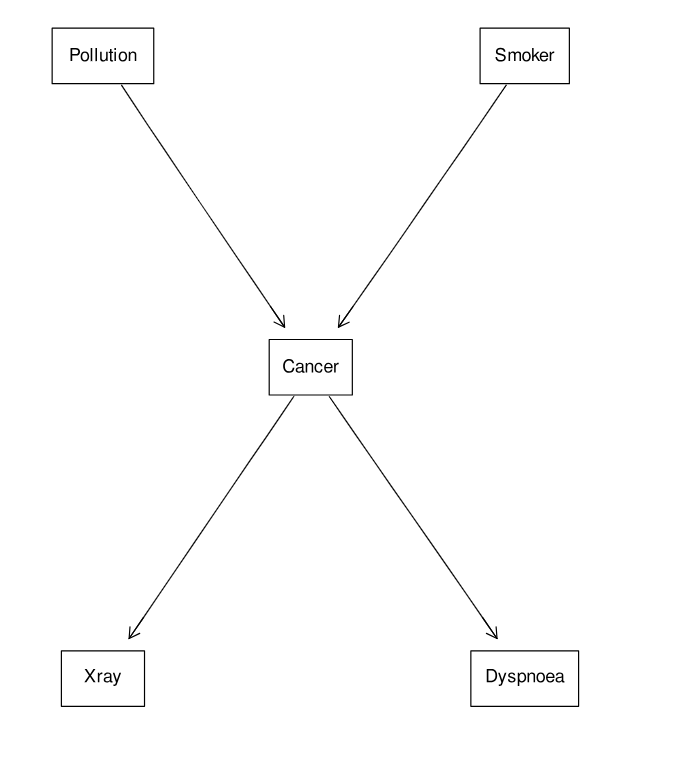
\includegraphics[width=\textwidth]{pic/img/bayesianNetworks/cancerNetwork.png}
			\caption{Red Bayesiana \cancerNetwork}
			\label{fig:cancer_network}
		\end{subfigure}
		\hfill
		\begin{subfigure}[b]{0.6\textwidth}
			\centering
			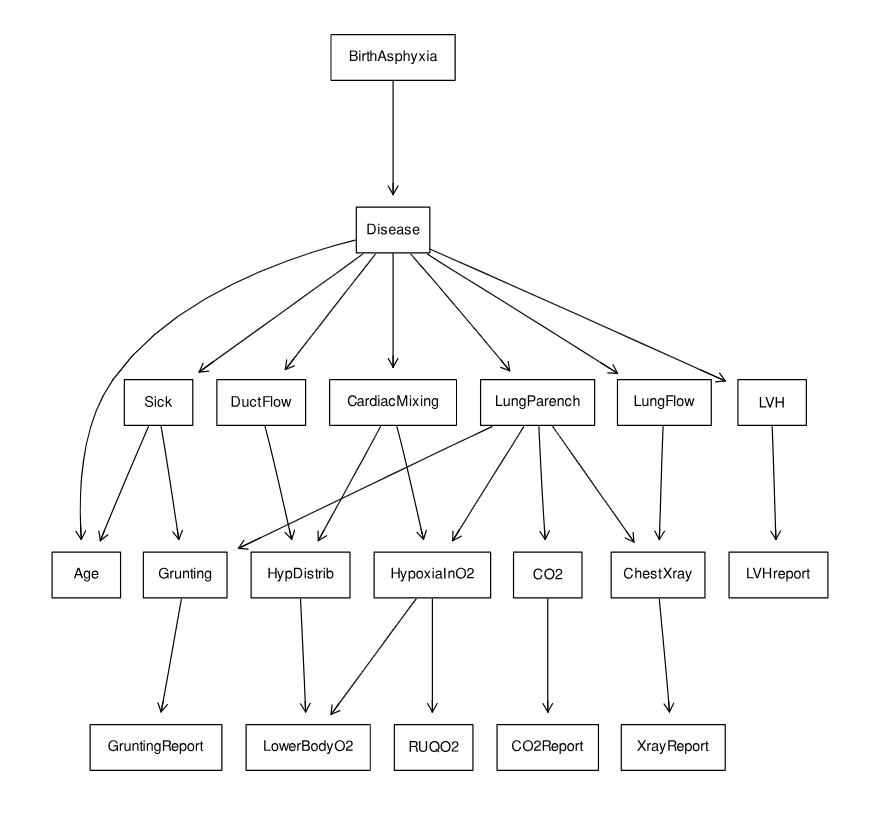
\includegraphics[width=\textwidth]{pic/img/bayesianNetworks/childNetwork.png}
			\caption{Red Bayesiana  \childNetwork}
			\label{fig:child_network}
		\end{subfigure}
		
		%\caption*{Ejemplos de redes bayesianas utilizadas en los experimentos.}
		\label{fig:bayesian_networks_combined}
	\end{figure}
\end{frame}

\begin{comment}
	\begin{frame}{Especificaciones del entorno experimental}
		\dificultyLevel{1}
		\begin{itemize}
			\item \textbf{Procesador:} Intel(R) Core(TM) i5-7500 CPU @ 3.40GHz
			\item \textbf{Memoria RAM:} 16 GB
			\item \textbf{Sistema operativo:} Ubuntu 22.04 LTS
			\item \textbf{Python:} Versi\'on 3.12
			\item \textbf{Paquetes:} \texttt{pgmpy}, \texttt{sklearn}, \texttt{networkx}, \texttt{shap}
		\end{itemize}
	\end{frame}
\end{comment}

\begin{frame}{Clases de equivalencia vs \'Ordenes topol\'ogicos}
	\dificultyLevel{2}
	\begin{mydefinition}[F\'ormula original de ASV]
		\[
			\assym_{M,e,\Pr}(x_i) = \frac{1}{|topos(G)|} \sum_{\alert{\pi \in topos(G)}} w(\pi) \left( \charactheristicFunction(\pi_{<i} \cup \{i\}) - \charactheristicFunction(\pi_{<i}) \right)
		\]
	\end{mydefinition}
	\begin{mydefinition}[Heur\'istica con clases de equivalencia]
		\[
		\assym_{M,e,\Pr}(x_i) =\frac{1}{|\topo(G)|} \sum_{\alert{\equivalenceClass \in eqCl(G, x_i)}} (\charactheristicFunction(\toOr_{<i} \cup \{x_i\}) - \charactheristicFunction(\toOr_{<i})) * |\equivalenceClass|
		\]
	\end{mydefinition}
	\pause
	\vspace{-10px}
	M\'etricas:
	\begin{itemize}[<+->]
		\item \textbf{Cardinalidad} de los conjuntos $\Rightarrow$ cantidad de evaluaciones %de $\charactheristicFunction$
		\item \textbf{Tiempo} para construir $topos(G)$ vs $eqCl(G,x_i)$
	\end{itemize}
\end{frame}

\begin{frame}{Cantidad de Clases de equivalencia vs \'Ordenes topol\'ogicos}
	\dificultyLevel{2}
	\centering
	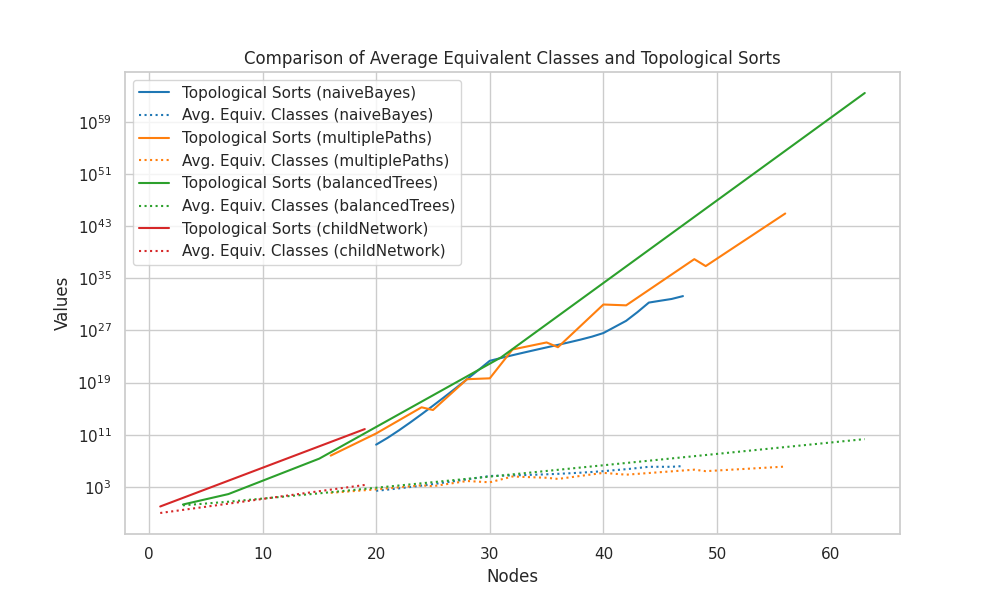
\includegraphics[width=0.95\linewidth]{pic/img/equivalentClassesVsToposorts.png}
	\captionof*{figure}{\scriptsize Cantidad de \'ordenes topol\'ogicos vs clases de equivalencia para distintas estructuras de grafos.}
\end{frame}

\begin{frame}{Tiempo de Clases de equivalencia vs \'Ordenes topol\'ogicos}
	
	\centering
	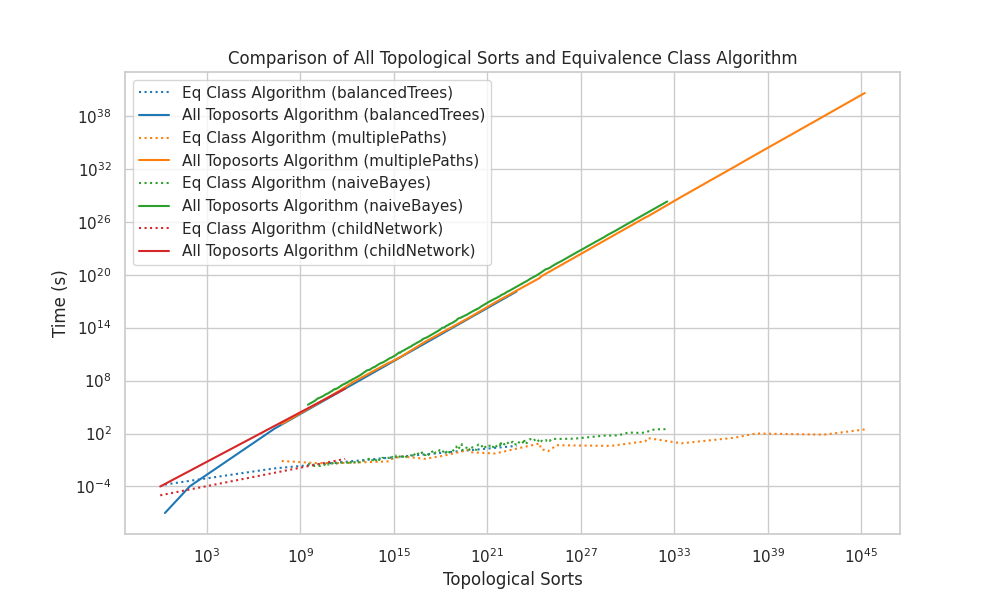
\includegraphics[width=\linewidth]{pic/img/equivalentClassesVsAllToposorts_time.png}
	\captionof*{figure}{\scriptsize Tiempo de clases vs topol\'ogicos usando el algoritmo de Knuth (networkx)}
	
\end{frame}

\begin{frame}{Comparaci\'on ASV vs SHAP (\cancerNetwork)}
	\dificultyLevel{2}
	\centering
	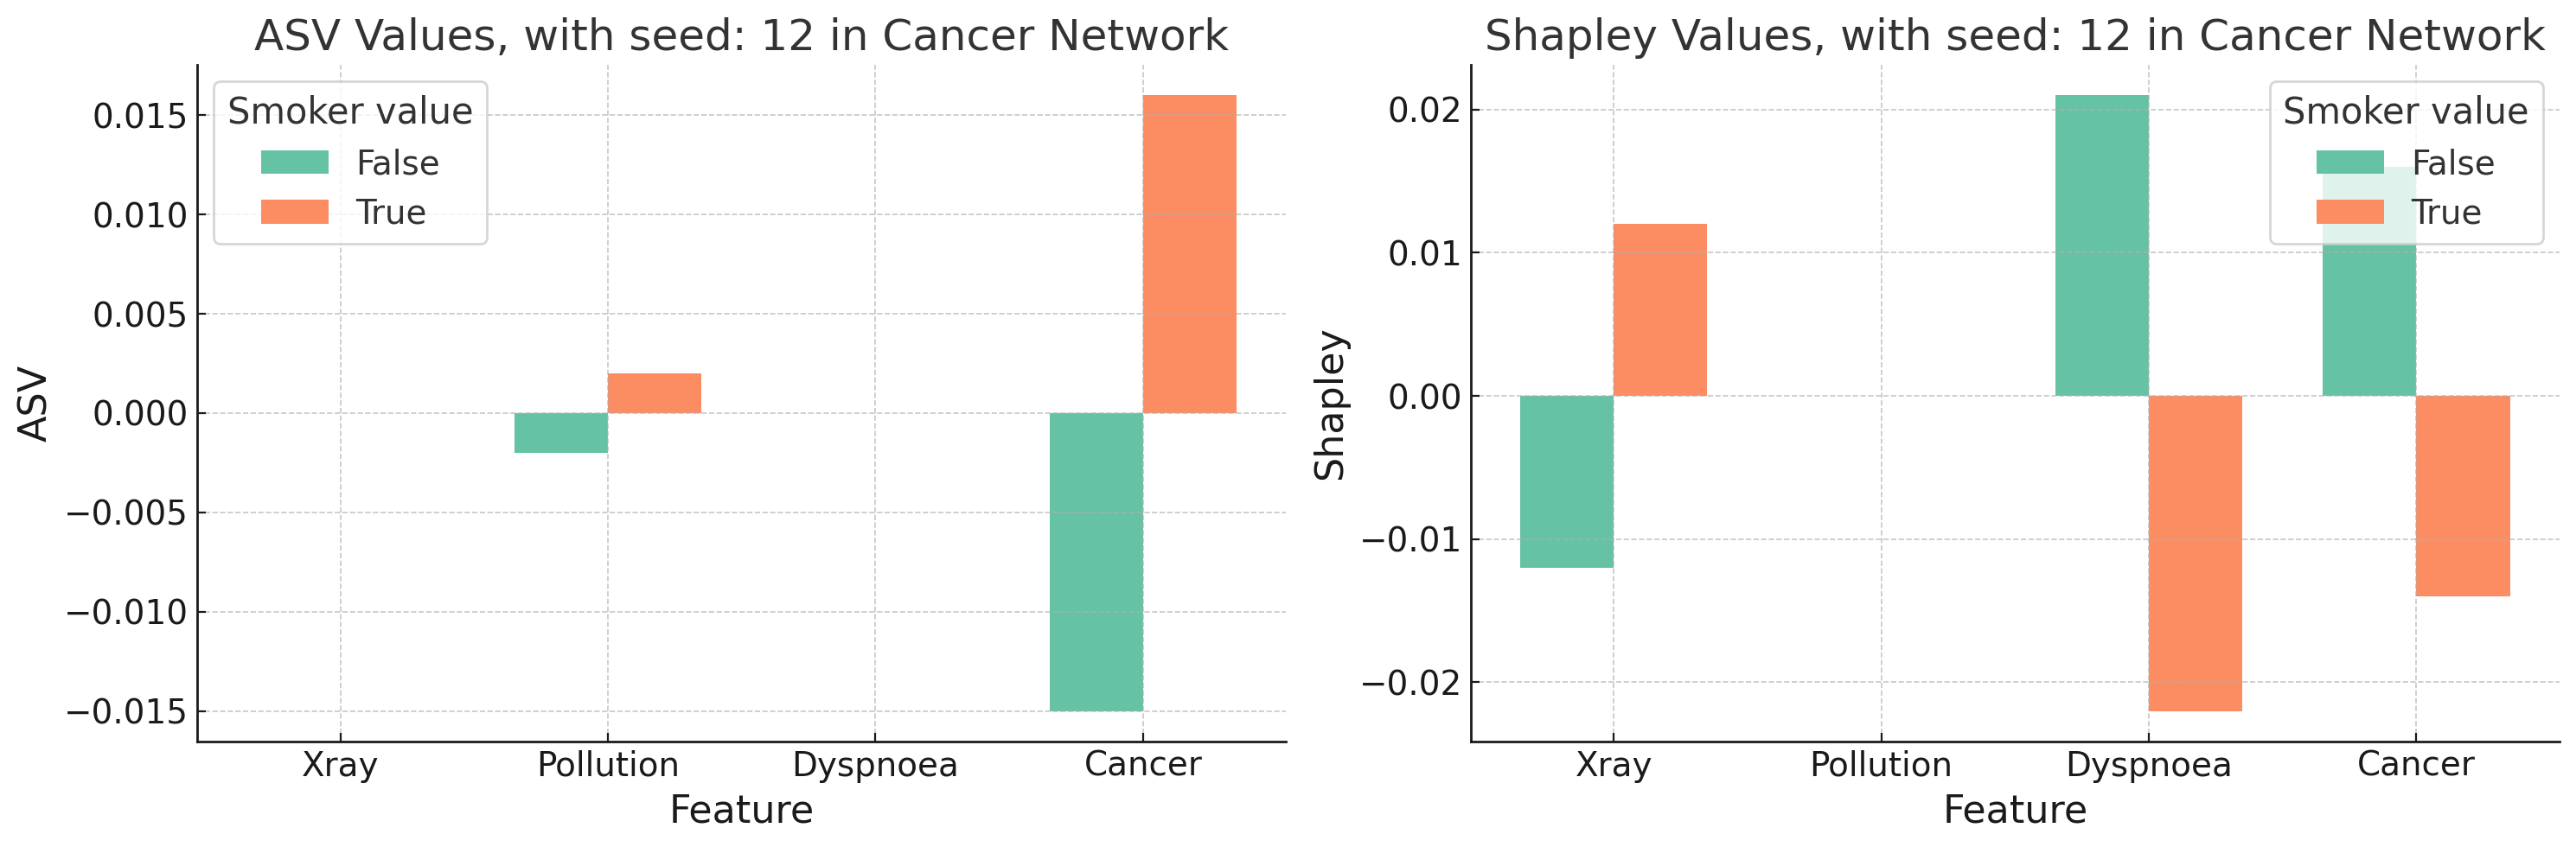
\includegraphics[width=1\linewidth]{pic/img/asvResults/cancerASVAndShapleyExactASVAndShapley.png}
	\captionof*{figure}{Comparación de los valores obtenidos por $ASV$ y $SHAP$ para las variables de la red \cancerNetwork}

\end{frame}

\begin{frame}{Variaci\'on de probabilidad para \texttt{Smoker}}
	\dificultyLevel{2}
	\centering
	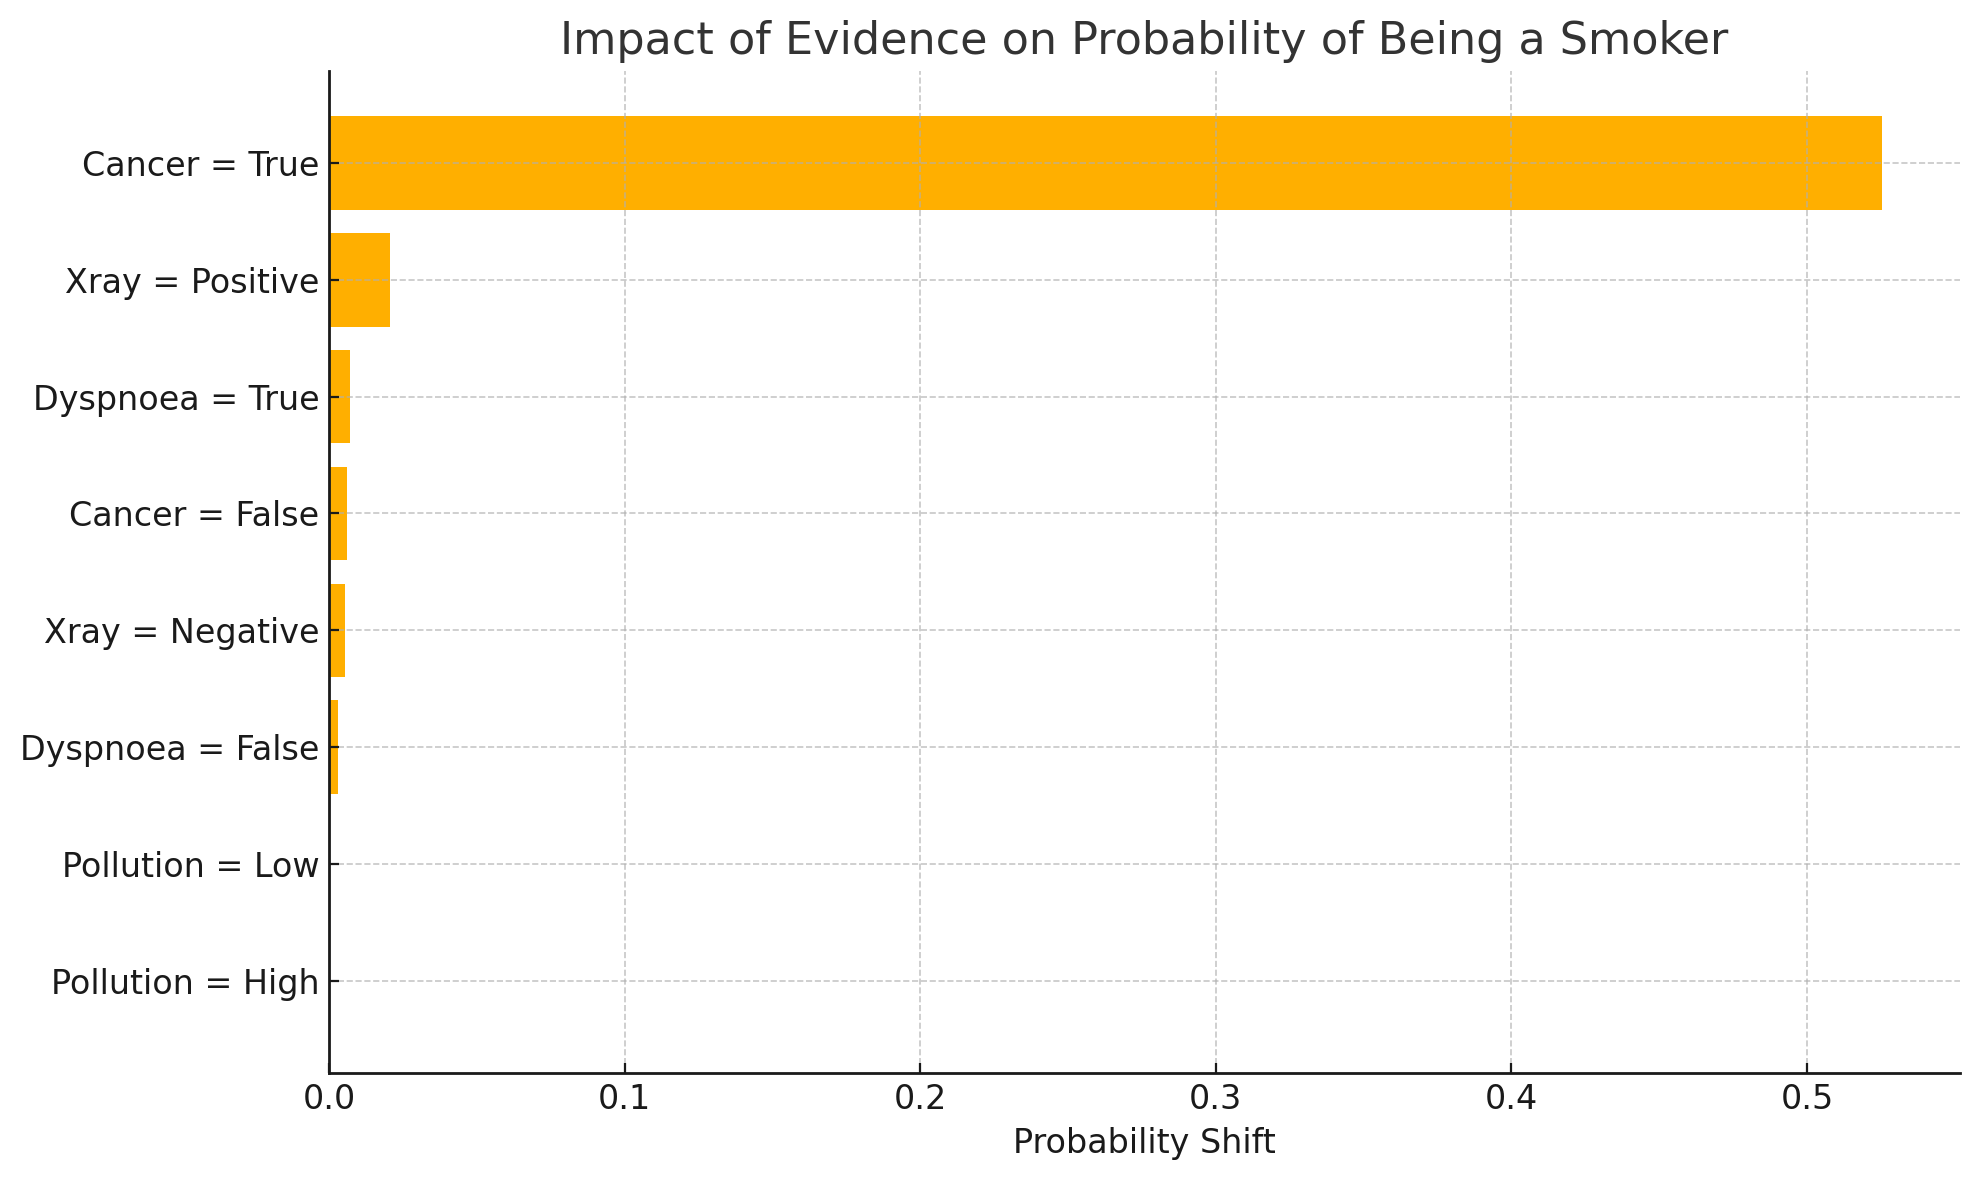
\includegraphics[width=0.95\linewidth]{pic/img/asvResults/probabilityShift.png}
	\captionof*{figure}{\scriptsize Métrica que analiza cuánto varía la probabilidad de \texttt{Smoker} en base a la evidencia introducida.}
\end{frame}

\begin{frame}{Comparaci\'on ASV vs SHAP (\childNetwork)}
	\dificultyLevel{2}
	\centering 
	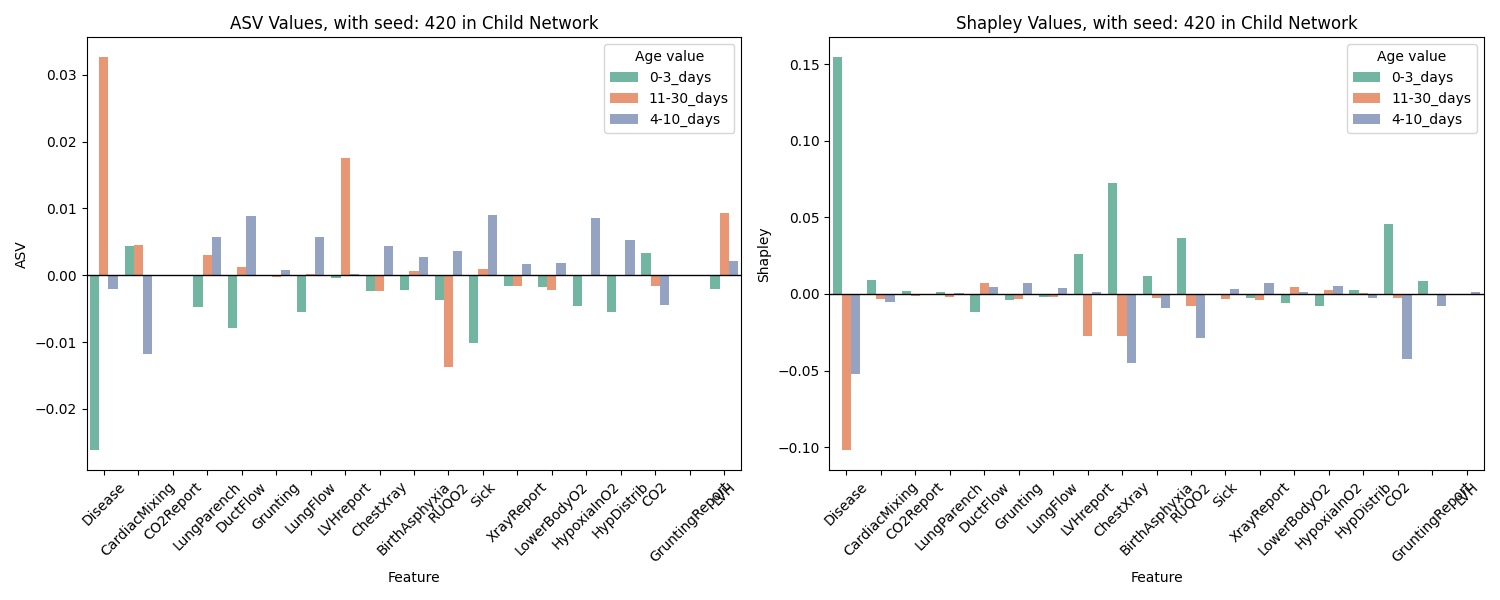
\includegraphics[width=0.95\linewidth]{pic/img/asvResults/childASVAndShapleyExactASVAndShapley.png}
	\vspace{0.5em}
	\begin{itemize}[<+->]
		\item $ASV$ identifica \texttt{Sick}, \texttt{DuctFlow}, \texttt{Disease}.
		\item $SHAP$ sólo logra detectar \texttt{Disease}.
		%\item Mayor intersecci\'on entre $ASV$ y Probability Shift.
	\end{itemize}
\end{frame}

\begin{frame}{Child: ASV exacto vs ASV aproximado (1000 muestreos)}
	\dificultyLevel{2}
	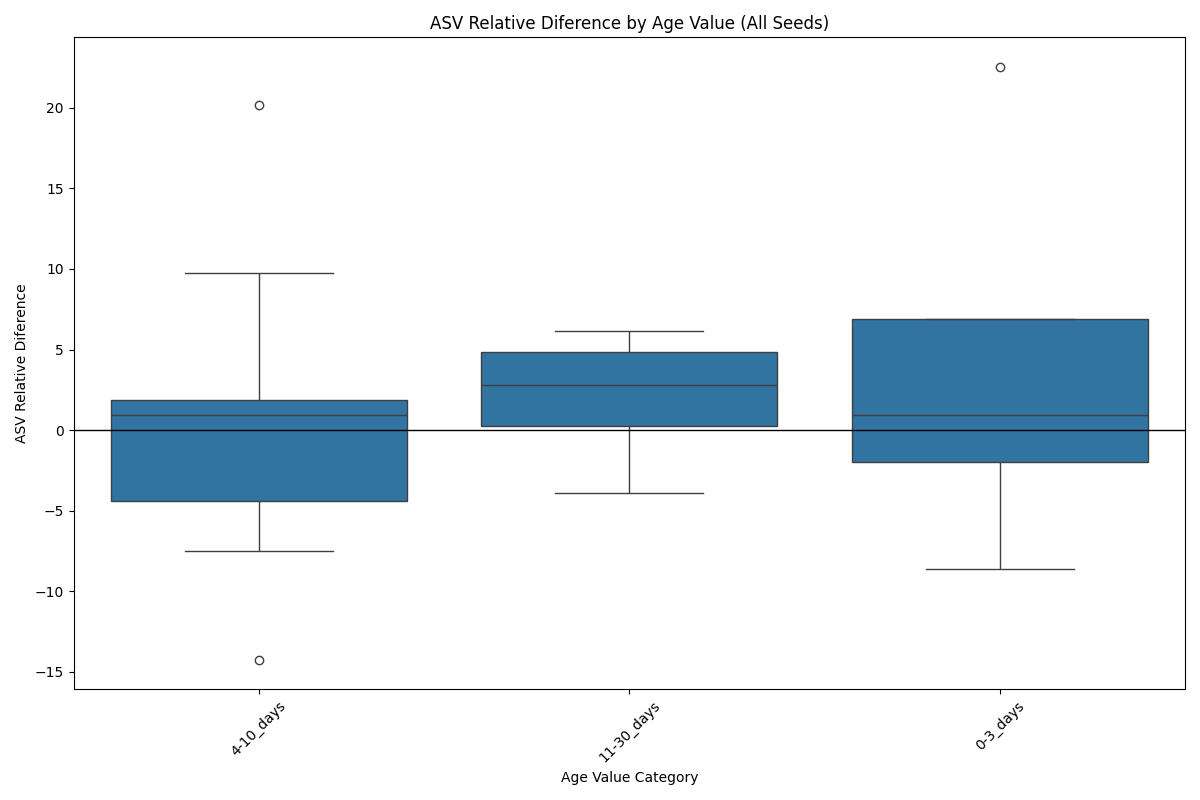
\includegraphics[width=0.8\linewidth]{pic/img/asvResults/ChildAllSeedsASVBoxplot.png}
	\vspace{0.5em}
	\begin{itemize}
		\item Error absoluto $< 5\%$ para $ASV > 0.01$.
		\item Aproximaci\'on razonable sin samplear una gran cantidad de órdenes.
	\end{itemize}
\end{frame}
